\definecolor{darkblue}{rgb}{0.00,0.00,0.65}       % rgb(0,0,126)
\definecolor{darkgreen}{RGB}{0,100,0}  % rgb(0,100,0)
\definecolor{darkred}{RGB}{174,0,0}        % rgb(174,0,0)

% - ``MALIN: Multi-Arm bandit Learning for Iot Networks with GRC: A TestBed Implementation and Demonstration that Learning Helps'', demo at ICT, and the companion paper ``GNU Radio Implementation of MALIN: "Multi-Armed bandits Learning for Internet-of-things Network"'', see https://hal.inria.fr/hal-02006825

\graphicspath{{2-Chapters/4-Chapter/IEEE_WCNC_2019__DemoICT.git/pictures/}}

In this Section, we present a demonstration showed at the International Conference on Telecommunication (ICT) in June $2018$ \cite{Besson2018ICT,Besson2019WCNC}, implementing a proof-of-concept of the model previously presented in Section~\ref{sec:4:firstModel}.

We implement an IoT network the following way: one gateway, one or several intelligent (\emph{i.e.}, learning) objects, embedding the proposed solution,
and a traffic generator that emulates radio interference from many other objects.
Intelligent objects communicate with the gateway with a wireless ALOHA-based protocol, which does not require any specific overhead for the learning.
%
Similarly to the previous Section, network access is modelled as a discrete sequential decision making problem, and using the framework and algorithms from MAB learning, we show that intelligent objects can improve their access to the network by using low complexity and decentralized algorithms, such as \UCB{} and Thompson Sampling.
%
This solution could be added in a straightforward and costless manner in LoRaWAN networks, just by adding this feature in some or all the devices, without any modification on the network side.


% ----------------------------------------------------------------------
\subsection{Context of this demonstration}
\label{sub:42:motivation}
% ----------------------------------------------------------------------

We describe the way we implemented a demo where we evaluate MAB algorithms, used in combination with a pure ALOHA-based protocol, such as the ones employed in LPWAN.
This demonstration is the first implementation which aims at assessing the potential gain of MAB learning algorithms in IoT scenarios.
%
We use a TestBed designed in 2017 by our team SCEE \cite[Appendix~3]{Bodinier17}, containing different USRP boards \cite{USRPDocumentation}, controlled by a single laptop using GNU Radio \cite{GNURadioDocumentation},
and where the intelligence of each object corresponds to a learning algorithm, implemented as a GNU Radio block \cite{GNURadioCompanionDocumentation} and written in Python or \texttt{C++}.

In our demo, we consider a simple wireless network, consisting of one gateway (radio access point), and a certain interfering background traffic, assumed to be stationary (\emph{i.i.d.}), which is generated by end-devices communicating in other networks.
Some dynamic intelligent objects (end-user or autonomous objects) try to communicate with the gateway, with a low-overhead protocol. This communication can be done in different channels which are also shared by devices using other networks.
Once the gateway receives a packet transmitted by a dynamic device in one channel, it transmits back to it an acknowledgement in the same channel, after a fixed-time delay, as it is done in the LoRaWAN standard.
This \emph{ACK} allows the device to learn about the channel quality and thus, to use learning algorithms for the purpose of best channel selection.

In this demo, we can generate scenarios with different parameters (number of channels, interfering traffic, etc) in order to evaluate the performance of learning in various settings.
Moreover, we compare the performance of learning with that of the random uniform access to channels, which is the current state-of-the-art of commercial LPWAN solutions.
%
This allows to check that in case of uniform traffic, when there is nothing to learn, the intelligent objects at least do not reduce their successful communication rate in comparison to the naive objects.
This also shows that in case of non-uniform stationary traffic, the MAB learning algorithms indeed help to increase the global efficiency of the network by improving the success rate of the intelligent objects.

We refer to Section~\ref{sec:2:famousMABalgorithms} which presented two bandit algorithms, \UCB{} and Thompson Sampling,
which are both known to be efficient for stationary \emph{i.i.d.} rewards and are shown to be useful in our setting (in Section~\ref{sec:42:results}).
Then we discuss the relevance of a MAB model for our IoT application.


\paragraph{Outline}

The rest of this Section is organized as follows.
Our implementation is presented in Section~\ref{sub:42:implementation}, with details about the user interface, and results are given in Section~\ref{sub:42:results}.


% ----------------------------------------------------------------------
\subsection{GNU Radio implementation}
\label{sub:42:implementation}
% ----------------------------------------------------------------------

In this Section, we present our implementation of MAB algorithms in the model of IoT networks presented in Section~\ref{sub:41:systemModel}.
We first describe the simplified physical layer of this demo, then we present our GNU Radio implementation.


\paragraph{Physical layer and protocol}

We implement a PHY/MAC layers solution in order to improve the performance of IoT communications in unlicensed bands. We could have used any physical layer and any ALOHA-based protocol.
We choose to implement our own physical layer and protocol, for both clarity and conciseness.

Regarding the physical layer, we consider a QPSK constellation. Moreover, we use simplified packets composed of two parts.
The first part is the \emph{preamble} which is used for the purpose of synchronization (phase correction).
Then, we have the \emph{index} of the user, which is a sequence of QPSK symbols.
For example, this index can be a simple QPSK symbol ($\pm1\pm1j$).
Once the gateway receives an uplink packet, it detects this index and transmits an acknowledgement which has the same frame structure, but where the index is the conjugate of the index of the uplink packet (\emph{e.g.}, $1+j \mapsto 1-j$).
Thanks to this index, we can have several devices communicating with the same gateway.

In turn, the end-device that receives the acknowledgement demodulates it, and checks if the index is the conjugate of its own index.
In this case, the \emph{ACK} was for him, and it knows that its packet has been received and decoded correctly by the gateway.


\paragraph{Equipment}
% Boards and versions
We use USRP N210 boards \cite{USRPDocumentation}, from Ettus Research (National Instrument),
with version $4$ of their FPGA system and version $5.1$ of the RBX system.
As illustrated in Figure~\ref{fig:42:our_demo}, our implementation is composed of at least $3$ USRP.
The gateway, a USRP which emulates the interfering traffic, and at least one dynamic device.
% Cables and laptop
% Osef

\begin{figure}[!t]
    \centering
    \includegraphics[width=0.70\linewidth]{our-demo.eps}
    \caption{Schematic of our implementation that presents the role of each USRP card.}
    \label{fig:42:our_demo}
\end{figure}

The boards have their own power supply, and are all connected to a local Ethernet switch, itself connected to a single laptop, running GNU/Linux and Ubuntu.
% Octoclock
To ease the synchronization in both time and frequency between the boards representing the dynamic objects and the gateway, we use an Octoclock \cite{OctoclockProduct}, also by Ettus Research,
% https://www.ettus.com/product/details/OctoClock-G
and coaxial cables connecting every card to the Octoclock for time (PPS) and frequency synchronization, but this is not mandatory.

\begin{figure}[!t]
    \centering
    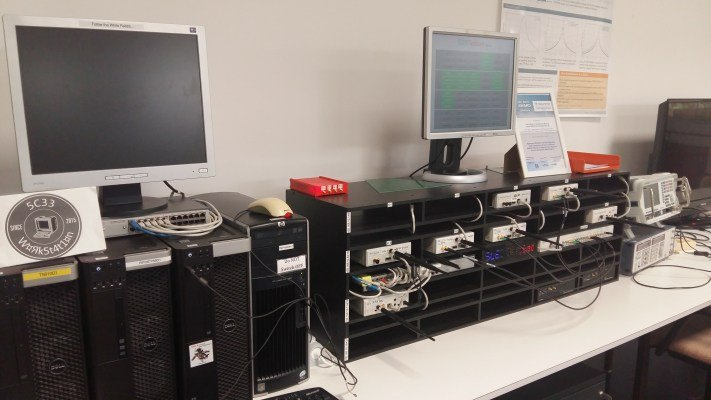
\includegraphics[width=0.65\linewidth]{SCEE_TestBed1.jpg}
    \vspace*{20pt}
    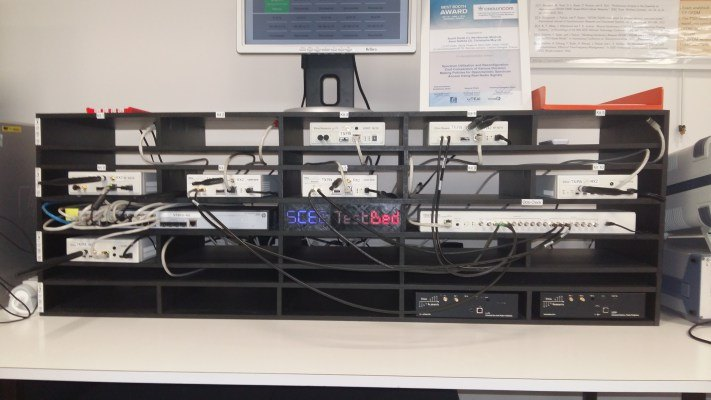
\includegraphics[width=0.65\linewidth]{SCEE_TestBed2.jpg}
    \caption{Two pictures showing the SCEE testbed \cite[Appendix~3]{Bodinier17}.}
    \label{fig:42:photosSCEETestBed}
\end{figure}


\paragraph{Implementation}

We used GNU Radio Companion (GRC, version $3.7$, $2017$),
and for the demonstration the laptop runs
one GRC design to configure and control each USRP card.
As such, a single laptop can run in parallel the control program of any number of boards\footnote{~Even if in practice, maximum efficiency is kept as long as there is not more than one GRC design by CPU core.}.

The GNU Radio software provides the framework and tools to build and run software radio or just general signal-processing applications.
GNU Radio applications are a flow-graph: a series of signal processing blocks connected together to describe a data flow.
For maximum efficiency, we wrote all of our blocks in \texttt{C++}.
These flow-graphs can be written in either C++ or the Python programming language. The GNU Radio infrastructure is written entirely in C++, and many of the user tools are written in Python.
GNU Radio Companion is a graphical UI used to develop GNU Radio applications:
GRC is effectively a Python code-generation tool.
when a flow-graph is compiled in GRC, a Python code is produced, which can be executed to connect to the USRP,
create the desired GUI windows and widgets, and create and connect the blocks in the flow-graph.


\paragraph{User Interface}

We have designed a user interface in order to visualize the results obtained  with our experimental demonstration. This user interface is shown in Figure~\ref{fig:42:UI}.
We can see that it is made of three parts, one for each USRP, as highlighted in \textcolor{darkred}{red}:

\begin{figure}[!t]
    \centering
    \includegraphics[width=0.80\textwidth]{UI.eps}
    \caption{User interface of our demonstration.}
    \label{fig:42:UI}
\end{figure}


% \begin{enumerate}[leftmargin=6mm]
    % \item[(1)]
$(1)$ The first part is the interface of the IoT traffic generator, where we see the traffic generated by this USRP, presented in a waterfall view in the time vs frequency domain.

    % \item[(2)]
$(2)$ The second part is the interface of the intelligent device which is made of four parts.
At the top left, we observe the constellation of the transmitted packet \emph{(a)}.
At the bottom left, we have a time/frequency view of the lasts packets transmitted by the object \emph{(b)}.
We can see, in this view that the object transmitted its last $9$ packets in the two best channels (channel $\#3$ and $\#4$).
Then, at the top right of this interface \emph{(c)}, we can see the traffic observed by this device, where we have the interfering traffic (\textcolor{darkgreen}{green}), the uplink packets transmitted by this object (\textcolor{darkred}{red}) and the acknowledgements sent by the gateway (\textcolor{darkblue}{blue}).
Finally, at the bottom right \emph{(d)}, we have four histograms showing the performance indicators of the chosen MAB algorithm (number of transmissions, number of successful transmissions, UCB indexes and success rates, in each channel).

    % \item[(3)]
$(3)$ The last part is the interface of the gateway, where we can see the traffic observed by the gateway \emph{(a)} and the channels in which the last acknowledgements have been sent \emph{(b)}.
% \end{enumerate}


% ----------------------------------------------------------------------
\subsection{Numerical results}
\label{sec:42:results}
% ----------------------------------------------------------------------

We compare the two algorithms described in Section~\ref{sec:2:famousMABalgorithms} against a uniform access algorithm, that uniformly selects its channel at random.
Three objects are compared by their mean successful communication rates, on a horizon of $2000$ communication slots, and were using three algorithms: uniform random access (in \textcolor{cyan}{cyan}), Thompson Sampling (in \textcolor{green}{green}) and \UCB{} (in \textcolor{red}{red}).
Figure~\ref{fig:42:plot_datafile_append_Uniform_vs_UCB_vs_TS} shows the results averaged on $10$ repetitions using the same conditions.
%
Each experiment takes about half a day,
as we make objects generate one message every $5$ seconds, in order to artificially speed up the process and with no loss of generality (as we are using real hardware).
Learning can be useful only when there is a large enough difference between ``good'' and ``bad'' channels,
Each object was learning to access $4$ different non-overlapping channels, that we chose to have occupancy rates of $[15\%, 10\%, 2\%, 1\%]$.
% They did not overlap each other, as
When facing the same stationary background traffic, we see that the learning objects are both very quickly more efficient than the naive uniform object.
We obtain an improvement in terms of successful communication rate from $40\%$ to about $60\%$ in only $100$ communications (about $16\;\mathrm{min}$), and up-to $80\%$ in only $400$ communications.
%
In stationary environments, both the TS and \UCB{} algorithms are very efficient and converge quickly, resulting in a very strong decrease in collisions and failed communication slots. \UCB{} is faster to learn but eventually TS gives a (slightly) better average performance.

Similar results are obtained for overlapping channels, when dynamic devices are learning in the presence of multiple devices, all using the same learning algorithm.
Empirical results confirm the simulations presented in Section~\ref{sec:4:firstModel} (see Figure~\ref{fig:41:perf_learning}).
Such results are very encouraging, and illustrate well the various strong possibilities of MAB learning applied to IoT networks.


\begin{figure}[!t]
	\centering
    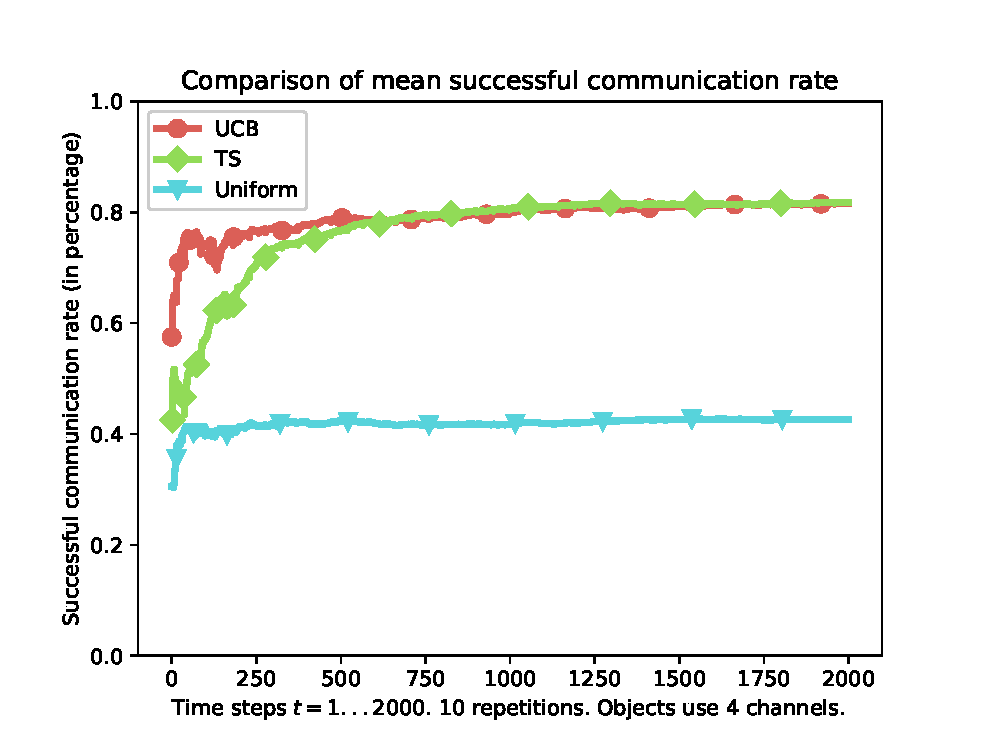
\includegraphics[height=9.0cm]{plot_datafile_append_Uniform_vs_UCB_vs_TS.eps}
    \caption{Less than $400$ communication slots (\emph{i.e.}, less than $100$ trials in each channel) suffice for the two learning objects to reach a successful communication rate close to $80\%$, which is \textbf{twice as much} as the non-learning (uniform) object, which stays around $40\%$ of success. Similar gains of performance were obtained in many different scenarios.}
    \label{fig:42:plot_datafile_append_Uniform_vs_UCB_vs_TS}
\end{figure}

% \begin{figure}[!t]
% 	\centering
%     \begin{subfigure}[b]{0.46\textwidth}
%         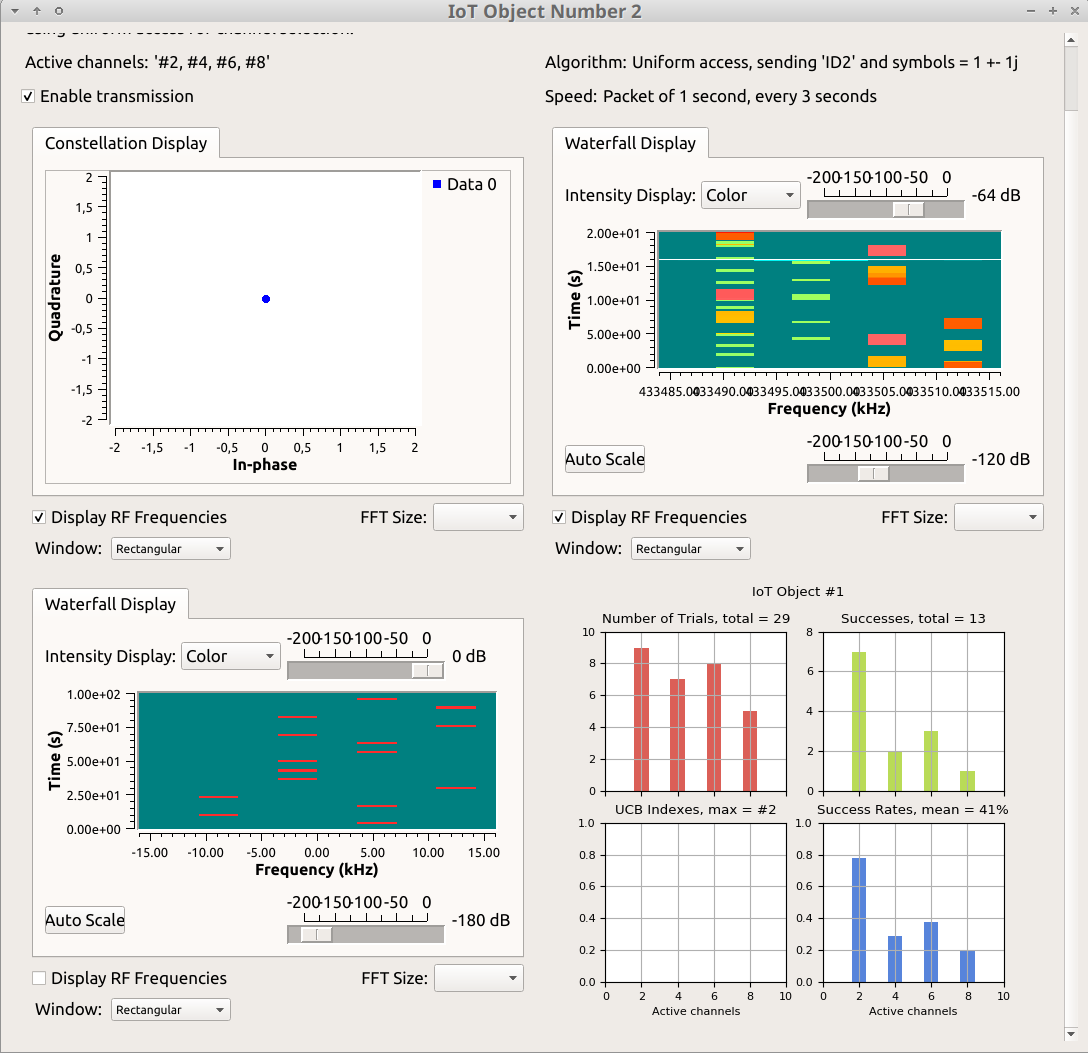
\includegraphics[height=7cm]{Object2_UniformAccess__UI.png}
%         %\caption{Object using uniform access.}
%         \label{fig:42:comparing_UniformAccess_and_UCB__1}
%     \end{subfigure}
%     ~ %add desired spacing between images, e. g. ~, \quad, \qquad, \hfill etc.
%       %(or a blank line to force the subfigure onto a new line)
%     \begin{subfigure}[b]{0.46\textwidth}
%         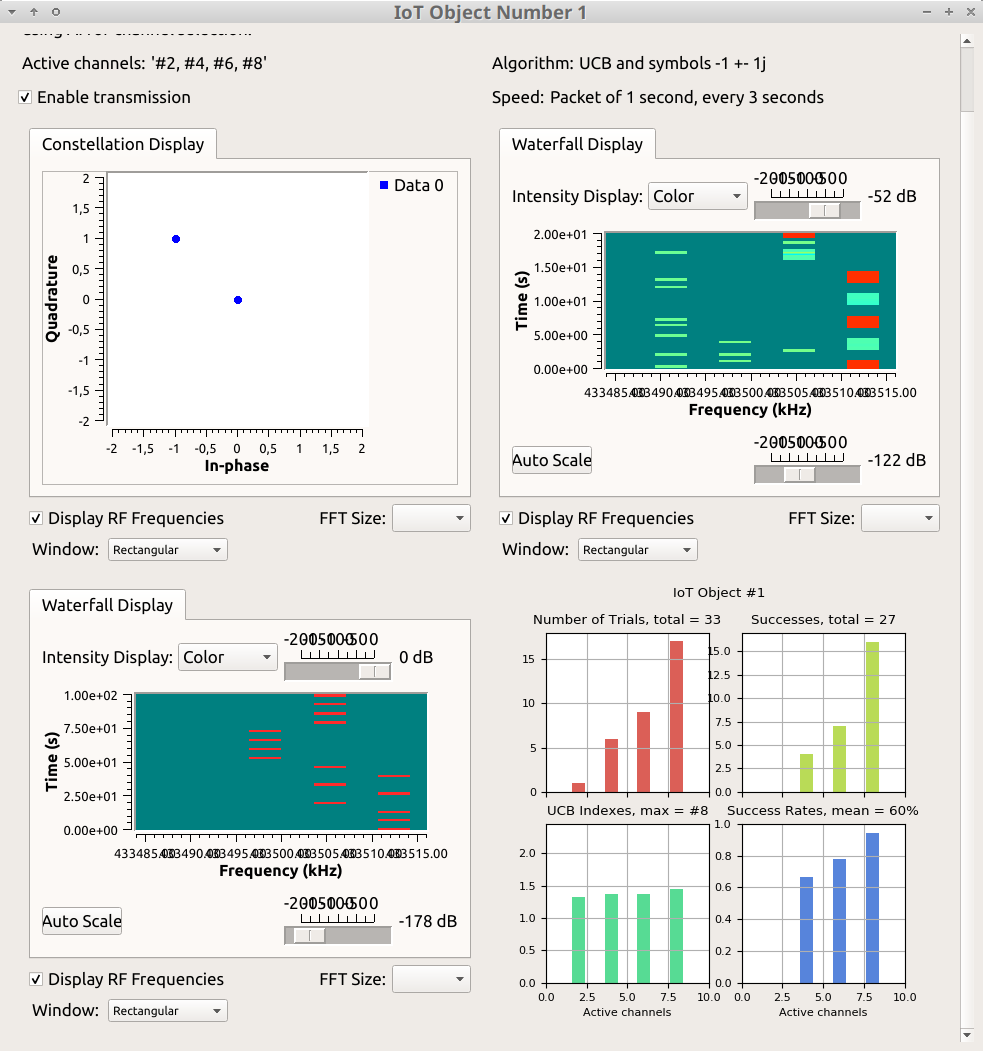
\includegraphics[height=7cm]{Object1_UCB__UI.png}
%         %\caption{Object using UCB.}
%         \label{fig:42:comparing_UniformAccess_and_UCB__2}
%     \end{subfigure}
% \caption{Comparing the success rate of an object using uniform access (left, $41\%$ of success here) and an object using the UCB algorithm (right, already $60\%$ of success). We see the learning object being much more present in the channels $\#4$ and $\#3$ (\textcolor{darkblue}{blue chart}, bottom right corner), as these channels are the less perturbed by the random interfering traffic, in this example.}
% \label{fig:42:comparing_UniformAccess_and_UCB}
% \end{figure}


\paragraph{Availability of data and materials}

The source code of our demonstration is fully available online, open-sourced under GPLv3 license, at
\href{https://bitbucket.org/scee_ietr/malin-multi-arm-bandit-learning-for-iot-networks-with-grc}{\texttt{bitbucket.org/scee\_ietr/\\malin-multi-arm-bandit-learning-for-iot-networks-with-grc/}}.

It contains both the GNU Radio Companion flowcharts and blocks, with ready-to-use \texttt{Makefiles} to easily compile, install and launch the demonstration.
The demonstration only requires a laptop and free tools,
as the laptop should run GNU/Linux and a distribution like Ubuntu or Debian.

\paragraph{Video}

A $6$-minute \textbf{video} showing our demonstration is available online at \texttt{\url{youtu.be/HospLNQhcMk}}.
It shows examples of $3$ dynamic devices learning simultaneously, confirming the results of Fig.~\ref{fig:42:plot_datafile_append_Uniform_vs_UCB_vs_TS} for overlapping channels.
It especially shows the connections between the USRP boards, the Octoclock, and the master laptop.

\paragraph{Special acknowledgment}

We acknowledge the work of two CentraleSup{\'e}lec students,
Cl{\'e}ment Barras and Th{\'e}o Vanneuville, for their GNU Radio project in Spring $2017$,
as we took inspiration in the GNU Radio code and the discussions we had at this time.
